% ===================================================================
%  Week 6 — Lecture Notes (Persian) — Frequency Domain (Fourier)
% ===================================================================
\documentclass[12pt,a4paper]{article}
% ===================================================================
%  Shared preamble for Persian lecture notes (Image Processing).
%  Compile with XeLaTeX.  Body = Persian (RTL), code/math = LTR.
% ===================================================================

\usepackage{geometry}
\geometry{a4paper,margin=2.4cm}
\usepackage{amsmath,amssymb}
\usepackage{graphicx}
\usepackage{xcolor}
\usepackage{listings}
\usepackage{tcolorbox}
\usepackage{booktabs}
\usepackage{array}
\usepackage{enumitem}
\usepackage{hyperref}
\tcbuselibrary{skins,breakable}

% ---- Persian / RTL --------------------------------------------------
\usepackage{xepersian}
\settextfont{IRNazli}
\setlatintextfont{Latin Modern Roman}
\setdigitfont{IRNazli}
% More generous leading + paragraph spacing (Persian reads better with air).
\linespread{1.5}
\setlength{\parskip}{0.7em}

% ---- Colours --------------------------------------------------------
\definecolor{coursePrimary}{HTML}{1B4965}
\definecolor{courseAccent}{HTML}{E76F51}
\definecolor{courseGood}{HTML}{2A9D8F}
\definecolor{courseBad}{HTML}{C0392B}
\definecolor{courseInfo}{HTML}{2980B9}
\definecolor{codeBg}{HTML}{F5F6FA}
\definecolor{codeKw}{HTML}{8E44AD}
\definecolor{codeStr}{HTML}{2A9D8F}
\definecolor{codeCom}{HTML}{7F8C8D}

\hypersetup{colorlinks=true,linkcolor=courseInfo,urlcolor=courseInfo,citecolor=courseInfo}

% ---- Code listings (Python built in) -------------------------------
\lstdefinestyle{course}{
  backgroundcolor=\color{codeBg},
  basicstyle=\ttfamily\small,
  keywordstyle=\color{codeKw}\bfseries,
  stringstyle=\color{codeStr},
  commentstyle=\color{codeCom}\itshape,
  numberstyle=\tiny\color{codeCom},
  numbers=left, numbersep=7pt,
  showstringspaces=false, breaklines=true,
  tabsize=4, columns=fullflexible, frame=single,
  rulecolor=\color{gray!30}, keepspaces=true, upquote=true, language=Python,
}
\lstset{style=course}
\lstdefinelanguage{bash}{
  keywords={cd,pip,python,venv,source,import}, sensitive=true,
  morecomment=[l]{\#}, morestring=[b]', morestring=[b]",
}
\newenvironment{ltrcode}{\begin{LTR}}{\end{LTR}}

% ---- Callout boxes (Persian titles) --------------------------------
\newtcolorbox{yaddasht}{colback=courseInfo!8,colframe=courseInfo,
  title={\textbf{یادداشت}},boxrule=0.6pt,right=6pt,left=6pt,breakable}
\newtcolorbox{nokte}{colback=courseAccent!10,colframe=courseAccent,
  title={\textbf{نکتهٔ کلیدی}},boxrule=0.6pt,right=6pt,left=6pt,breakable}
\newtcolorbox{hoshdar}{colback=courseBad!8,colframe=courseBad,
  title={\textbf{هشدار / دام}},boxrule=0.6pt,right=6pt,left=6pt,breakable}
\newtcolorbox{riyazi}{colback=coursePrimary!6,colframe=coursePrimary,
  title={\textbf{ریاضیات}},boxrule=0.6pt,right=6pt,left=6pt,breakable}
\newtcolorbox{tamrin}{colback=courseGood!8,colframe=courseGood,
  title={\textbf{تمرین}},boxrule=0.6pt,right=6pt,left=6pt,breakable}

% ---- Header helper --------------------------------------------------
\newcommand{\coursemeta}[2]{%
  \begin{center}
  {\large\textbf{پردازش تصویرِ کاربردی}}\\[2pt]
  {\color{coursePrimary}\rule{\linewidth}{1pt}}\\[4pt]
  {\Large\textbf{#1}}\\[3pt]
  {\small جزوهٔ درس — #2}
  \end{center}\vspace{4pt}
}


\begin{document}
\coursemeta{جلسهٔ ۶ — حوزهٔ فرکانس (فوریه)}{هفتهٔ ششم}

{\small\itshape مکملِ اسلایدهای انگلیسیِ جلسهٔ ۶. تصاویر و طیف‌ها از دیتاستِ واقعیِ شما (پلاک) تولید شده‌اند. هدف: دیدنِ تصویر به‌صورتِ مجموعِ موج‌ها، و حذفِ نویزِ دوره‌ای که در حوزهٔ مکانی تقریباً غیرممکن است.}

\vspace{0.5cm}
\tableofcontents
\vspace{1cm}

% ===================================================================
\section{چرا این جلسه}

جلسات ۳ تا ۵ در حوزهٔ \textbf{مکانی} (پیکسل و کرنل) کار می‌کردند. امروز حوزهٔ \textbf{فرکانس} را
یاد می‌گیریم: هر تصویر مجموعی از موج‌هاست. برخی عملیات اینجا بسیار ساده‌ترند، و \textbf{نویزِ
دوره‌ای} به‌سادگی حذف می‌شود. یک اسکنِ راه‌راه از کنتور در حوزهٔ مکانی تقریباً غیرقابلِ‌پاک‌سازی
است — اما در حوزهٔ فرکانس فقط چند نقطه است.

\subsection{شهودِ اولیه: چرا موج‌ها؟}

چرا باید تصویر را به موج‌ها بشکنیم؟ چون بسیاری از پدیده‌ها ذاتاً \emph{فرکانسی}‌اند: نویزِ دوره‌ای
یک فرکانسِ خاص است؛ لبه‌ها فرکانس‌بالا هستند؛ روشناییِ کلی فرکانس‌پایین است. وقتی مسئله را در زبانِ
فرکانس بیان کنید، راه‌حل اغلب بدیهی می‌شود: «راه‌راه‌ها را حذف کن» = «آن فرکانسِ خاص را صفر کن».

یک قیاسِ صوتی کمک می‌کند: صدا هم مجموعِ فرکانس‌هاست. یک اکولایزر (\lr{equalizer}) که باس یا تربل
را کم/زیاد می‌کند، دقیقاً یک فیلترِ فرکانسی است. حذفِ یک وزوزِ ۵۰ هرتزی از یک ضبط، همان فیلترِ
notch است که ما روی تصویر انجام می‌دهیم — اما در یک بُعد.

% ===================================================================
\section{ایدهٔ فوریه}

\textbf{فوریه}: هر تصویر را می‌توان مجموعِ سینوسی‌های دوبعدی با \textbf{فرکانس}، \textbf{جهت} و
\textbf{دامنهٔ} مختلف نوشت. فرکانس‌های پایین = تغییرِ آرام و نرم (روشناییِ کلی، شکل‌های بزرگ)؛
فرکانس‌های بالا = تغییرِ سریع (لبه، بافتِ ریز، نویز).

\begin{riyazi}
تبدیلِ فوریهٔ گسستهٔ دوبعدی (\lr{2D DFT}):
\[
F(u,v)=\sum_{x}\sum_{y} f(x,y)\,e^{-j2\pi(ux/W + vy/H)}
\]
$F(u,v)$ می‌گوید چقدر از موجی با فرکانسِ $(u,v)$ در تصویر هست.
\end{riyazi}

\subsection{طیفِ یک پلاکِ واقعی}

\begin{center}
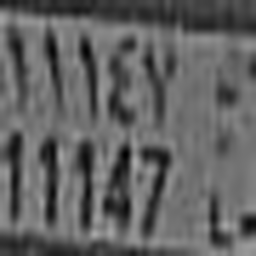
\includegraphics[width=0.4\linewidth]{../assets/gray.png}\quad
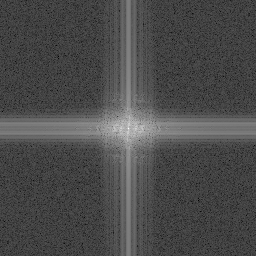
\includegraphics[width=0.4\linewidth]{../assets/spectrum.png}\\[2pt]
{\small چپ: تصویر (مکانی) — راست: طیفِ اندازه (لگاریتمی)}
\end{center}

\begin{itemize}
  \item مرکز = فرکانس‌های پایین (\lr{DC} = میانگینِ روشنایی). لبه‌ها = فرکانس‌های بالا.
  \item خط‌ها/نقاطِ روشن، جهت‌های غالب و ساختارِ تکرارشونده را آشکار می‌کنند.
\end{itemize}

\begin{nokte}
از \lr{log}ِ اندازه استفاده می‌کنیم تا چیزی ببینیم — جملهٔ \lr{DC} (میانگین) از بقیه بسیار
بزرگ‌تر است و بدونِ لگاریتم فقط یک نقطهٔ روشن در مرکز و بقیه سیاه می‌بینید.
\end{nokte}

\subsection{خواندنِ طیف}

\begin{itemize}
  \item \textbf{مرکز} میانگین است؛ انرژی معمولاً آنجا متمرکز است (تصاویرِ طبیعی عمدتاً فرکانس‌پایین‌اند).
  \item یک \textbf{جهتِ} قوی در تصویر $\rightarrow$ یک خطِ روشنِ \emph{عمود بر آن} در طیف.
  \item \textbf{الگوهای تکرارشونده} (راه‌راه، هافتون) $\rightarrow$ \textbf{پیک}‌های روشنِ منزوی خارج از مرکز.
\end{itemize}

% ===================================================================
\section{فیلترکردن در فرکانس}

\begin{center}
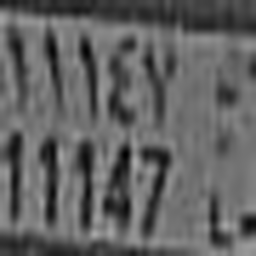
\includegraphics[width=0.3\linewidth]{../assets/gray.png}\quad
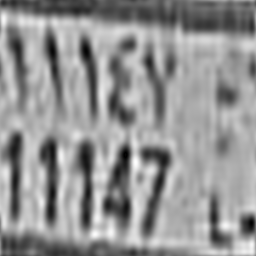
\includegraphics[width=0.3\linewidth]{../assets/lowpass.png}\quad
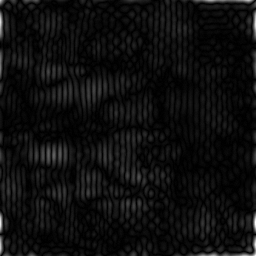
\includegraphics[width=0.3\linewidth]{../assets/highpass.png}\\[2pt]
{\small اصلی — پایین‌گذر (تاری) — بالاگذر (لبه)}
\end{center}

مرکز (فرکانس‌پایین) را نگه دارید $\rightarrow$ هموارسازی. مرکز را حذف کنید (بالا را نگه دارید)
$\rightarrow$ لبه. همان اثراتِ جلسهٔ ۳، اما با \emph{ماسک‌کردنِ} طیف.

\begin{riyazi}
\textbf{قضیهٔ کانولوشن}: کانولوشن در مکان $=$ ضرب در فرکانس:
$f * h \;\longleftrightarrow\; F\cdot H$.
\end{riyazi}

یک کانولوشنِ بزرگِ مکانی به یک ضربِ عنصربه‌عنصرِ ارزان در فرکانس تبدیل می‌شود. برای کرنل‌های بزرگ،
فیلترکردنِ مبتنی بر FFT بسیار سریع‌تر است ($O(N\log N)$ در برابرِ $O(N k^2)$). این هم \emph{چراییِ}
اینکه دیدِ مکانی و فرکانسی دو رویِ یک سکه‌اند.

\subsection{آزمایشِ هم‌ارزی: فرکانس در برابرِ مکان}

قضیهٔ کانولوشن می‌گوید تاریِ گاوسیِ مکانی و پایین‌گذرِ گاوسیِ فرکانسی باید نتیجهٔ یکسان بدهند. این
را می‌توان آزمایش کرد:

\begin{ltrcode}
\begin{lstlisting}[language=Python]
# spatial blur
spatial = cv2.GaussianBlur(gray, (0, 0), sigma=3)
# frequency low-pass with an equivalent Gaussian in frequency
F = np.fft.fftshift(np.fft.fft2(gray))
H = gaussian_lowpass(gray.shape, D0=...)   # matched cutoff
freq = np.abs(np.fft.ifft2(np.fft.ifftshift(F * H)))
# the two results are (nearly) identical
\end{lstlisting}
\end{ltrcode}

این هم‌ارزی نکتهٔ مهمی دارد: برای کرنل‌های \emph{کوچک} (مثلِ $5\times5$)، حوزهٔ مکانی سریع‌تر و
ساده‌تر است؛ برای کرنل‌های \emph{بزرگ} (مثلِ یک تاریِ $101\times101$)، حوزهٔ فرکانس (FFT) بسیار
سریع‌تر است. پس انتخابِ حوزه یک تصمیمِ مهندسیِ سرعت است، نه فقط سلیقه.

\begin{nokte}
اختلافِ کوچکِ عملی: نسخهٔ FFT فرض می‌کند تصویر \emph{تناوبی} است (لبهٔ راست به لبهٔ چپ می‌چسبد)،
که می‌تواند مصنوعاتِ مرزی بسازد. برای همین گاهی پیش از FFT، تصویر را با \lr{padding} یا پنجره‌گذاری
آماده می‌کنند. این یکی از تفاوت‌های ظریفِ نظریه و عمل است.
\end{nokte}

\subsection{فیلترِ ایده‌آل در برابرِ نرم (نوسان)}

یک برشِ تیزِ \textbf{ایده‌آل} (دایرهٔ سخت) باعثِ \textbf{نوسان} (\lr{ringing}) می‌شود — موج‌های
ریز نزدیکِ لبه‌ها. برش‌های نرم (\lr{Butterworth}، گاوسی) از نوسان جلوگیری می‌کنند — انتخابِ
معمول. مبادله: گزینش‌گریِ فرکانسیِ تیزتر $\leftrightarrow$ نوسانِ مکانیِ بیشتر.

% ===================================================================
\section{نویزِ دوره‌ای — کاربردِ ویژه}

\begin{center}
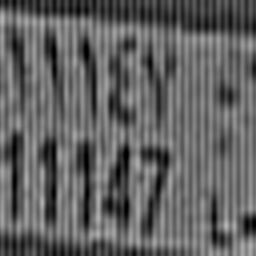
\includegraphics[width=0.3\linewidth]{../assets/periodic_noisy.png}\quad
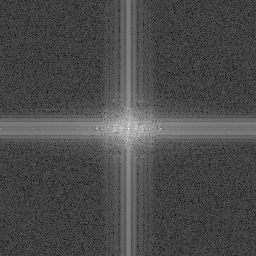
\includegraphics[width=0.3\linewidth]{../assets/periodic_spectrum.png}\quad
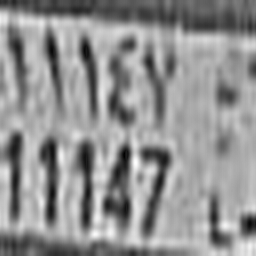
\includegraphics[width=0.3\linewidth]{../assets/periodic_fixed.png}\\[2pt]
{\small نویزِ راه‌راه — طیف: دو پیکِ روشن — پس از notch: تمیز}
\end{center}

\begin{nokte}
راه‌راه‌های تکرارشونده در حوزهٔ مکانی کابوس‌اند — اما در فرکانس فقط دو نقطه‌اند. نقطه‌ها را صفر
کنید (فیلترِ \textbf{notch})، معکوس بگیرید، تمام. این تفاوتِ چشمگیرِ دو حوزه است.
\end{nokte}

\subsection{فیلترِ notch}

یک فیلترِ \textbf{notch} نواحیِ کوچکی از طیف (پیک‌های نویز) را صفر می‌کند و بقیه را نگه می‌دارد.
پیک‌ها را بیابید (نسبت به مرکز متقارن‌اند)، ماسکشان کنید، و تبدیلِ معکوس بگیرید. عالی برای خطوطِ
اسکن، الگوهای هافتون، تداخلِ حسگر — مصنوعاتِ واقعیِ اسناد. برای DocScan: اگر یک فرمِ اسکن‌شده الگوی
پس‌زمینهٔ تکرارشونده دارد، فیلترِ notch آن را تمیز حذف می‌کند.

\begin{ltrcode}
\begin{lstlisting}[language=Python]
F = np.fft.fftshift(np.fft.fft2(gray))     # to frequency, centre the DC
mag = 20*np.log(np.abs(F) + 1)             # log magnitude for display
mask = make_circle_mask(gray.shape, r=30)  # low-pass disc
out = np.abs(np.fft.ifft2(np.fft.ifftshift(F * mask)))  # back to spatial
\end{lstlisting}
\end{ltrcode}

\lr{fft2} $\rightarrow$ ماسک $\rightarrow$ \lr{ifft2}. کلِ گردشِ کارِ فرکانسی در سه گام.

% ===================================================================
\section{یک مثالِ یک‌بعدی برای شهود}

فوریهٔ دوبعدی سخت به‌نظر می‌رسد؛ با یک‌بعدی شروع کنیم. تصور کنید یک سیگنالِ یک‌بعدی که مجموعِ دو
موجِ سینوسی است: یکی با فرکانسِ پایین (آرام) و یکی با فرکانسِ بالا (سریع). تبدیلِ فوریه این را به
دو پیک تبدیل می‌کند: یکی نزدیکِ صفر (موجِ آرام) و یکی دورتر (موجِ سریع). ارتفاعِ هر پیک = دامنهٔ
آن موج.

\begin{riyazi}
اگر $f(x) = 3\sin(2\pi \cdot 2x) + \sin(2\pi \cdot 10x)$، طیف دو پیک دارد: یکی در فرکانسِ ۲ با
ارتفاعِ ۳، و یکی در فرکانسِ ۱۰ با ارتفاعِ ۱. تبدیلِ فوریه دقیقاً «چه موج‌هایی، با چه دامنه‌ای» را
بازمی‌گرداند.
\end{riyazi}

\begin{nokte}
حالا تصویرِ دوبعدی را تعمیمِ همین بدانید: به‌جای فرکانس در یک بُعد، موج‌هایی با فرکانس \emph{و
جهت} داریم. یک راه‌راهِ عمودی = یک موج در جهتِ افقی. یک بافتِ قطری = موج‌هایی در جهتِ قطری. طیف،
نقشهٔ همهٔ این موج‌هاست.
\end{nokte}

% ===================================================================
\section{طراحیِ فیلترِ فرکانسی}

سه نوعِ رایجِ فیلترِ پایین‌گذر (برای بالاگذر، متمم‌شان را بگیرید):

\begin{itemize}
  \item \textbf{ایده‌آل}: یک دایرهٔ سخت با شعاعِ $D_0$؛ درونش ۱، بیرونش ۰. تیز اما نوسان می‌سازد.
  \item \textbf{باترورث} (\lr{Butterworth}): برشِ تدریجی که تیزی‌اش با «مرتبه» تنظیم می‌شود. تعادلِ خوب.
  \item \textbf{گاوسی}: نرم‌ترین برش؛ هیچ نوسانی نمی‌سازد.
\end{itemize}

\begin{riyazi}
فیلترِ گاوسیِ پایین‌گذر در فرکانس: $H(u,v) = e^{-D^2(u,v)/(2D_0^2)}$، که $D(u,v)$ فاصله از مرکز
و $D_0$ فرکانسِ برش است. جالب: تبدیلِ فوریهٔ یک گاوسی، خودش یک گاوسی است — برای همین تاریِ
گاوسیِ مکانی و پایین‌گذرِ گاوسیِ فرکانسی معادل‌اند.
\end{riyazi}

\begin{hoshdar}
مبادلهٔ اساسی: هرچه فیلتر در فرکانس تیزتر باشد، در مکان پهن‌تر و نوسانی‌تر است (اصلِ عدمِ قطعیت).
یک برشِ کاملاً تیز در فرکانس، یک \lr{sinc}ِ بی‌نهایت با نوسان در مکان است. برای همین برش‌های نرم
(گاوسی/باترورث) در عمل بهترند.
\end{hoshdar}

% ===================================================================
\section{تمرینِ کلاسیِ وسط‌جلسه (۱۰ دقیقه)}

\begin{tamrin}
برای هر تصویر، طیفِ اندازه‌اش چه شکلی است؟ (۱) یک تصویرِ خاکستریِ کاملاً تخت. (۲) راه‌راه‌های
سیاه‌وسفیدِ عمودی. (۳) عکسی با بافتِ ریزِ فراوان در برابرِ یک گرادیانِ نرم. (۴) برای تشخیصِ یک
الگوی اسکنِ تکرارشونده، کجای طیف را نگاه می‌کنید؟
\end{tamrin}

\textbf{جمع‌بندی:} (۱) تخت $\rightarrow$ یک نقطهٔ واحد در مرکز (فقط \lr{DC})؛ (۲) راه‌راهِ عمودی
$\rightarrow$ دو نقطهٔ متقارن روی محورِ افقی (یک فرکانس)؛ (۳) بافتِ ریز $\rightarrow$ انرژیِ زیاد
دور از مرکز، نرم $\rightarrow$ انرژیِ چسبیده به مرکز؛ (۴) دنبالِ پیک‌های روشنِ منزویِ خارج از مرکز
بگردید — آن ساختارِ دوره‌ای است. طیف نقشهٔ «چقدر از هر موج» است؛ خواندنش با تمرین شهود می‌شود.

% ===================================================================
\section{فیلترِ notch گام‌به‌گام}

بیایید حذفِ نویزِ دوره‌ای را کامل انجام دهیم:

\begin{enumerate}
  \item تصویرِ نویزیِ راه‌راه را به فرکانس ببرید و طیف را ببینید.
  \item پیک‌های روشنِ خارج از مرکز را بیابید (نویزِ دوره‌ای این‌ها را می‌سازد). چون تابعِ حقیقی است، پیک‌ها متقارن‌اند.
  \item یک ماسک بسازید که دایره‌های کوچکی دورِ آن پیک‌ها را صفر کند و بقیه را ۱ نگه دارد.
  \item ماسک را در طیف ضرب کنید و تبدیلِ معکوس بگیرید.
\end{enumerate}

\begin{ltrcode}
\begin{lstlisting}[language=Python]
F = np.fft.fftshift(np.fft.fft2(noisy))
mask = np.ones(F.shape, np.float32)
cy, cx = F.shape[0]//2, F.shape[1]//2
Y, X = np.ogrid[:F.shape[0], :F.shape[1]]
for peak in [cx-32, cx+32]:            # the two noise peaks
    d = np.sqrt((Y-cy)**2 + (X-peak)**2)
    mask[d < 6] = 0                    # zero a small disc around each
clean = np.abs(np.fft.ifft2(np.fft.ifftshift(F * mask)))
\end{lstlisting}
\end{ltrcode}

\begin{nokte}
نکتهٔ ظریف: \emph{اندازهٔ} دایره‌های notch مهم است — خیلی کوچک، نویز را کامل حذف نمی‌کند؛ خیلی
بزرگ، فرکانس‌های مفید را هم می‌برد و مصنوع می‌سازد. مثلِ همهٔ پارامترها، روی داده تنظیمش کنید.
\end{nokte}

% ===================================================================
\section{کاربردهای حوزهٔ فرکانس}

\begin{itemize}
  \item \textbf{حذفِ نویزِ دوره‌ای}: خطوطِ اسکن، هافتونِ روزنامه، تداخلِ برق.
  \item \textbf{تحلیلِ بافت}: جهت و تناوبِ یک بافت (پارچه، اثرِ انگشت) در طیف آشکار است.
  \item \textbf{فشرده‌سازی}: JPEG (DCT)، موجک‌ها.
  \item \textbf{تطبیقِ الگو}: همبستگیِ متقاطع در فرکانس سریع‌تر است.
  \item \textbf{واترمارک}: نهفتنِ اطلاعات در فرکانس‌های خاص.
\end{itemize}

\subsection*{چک‌لیستِ دام‌های این هفته}

\begin{itemize}
  \item فراموشیِ \lr{fftshift} (مرکزکردنِ DC) — طیف به‌هم‌ریخته و غیرقابلِ‌تفسیر.
  \item فراموشیِ \lr{log} برای نمایش — فقط یک نقطهٔ روشن در مرکز می‌بینید.
  \item برشِ فرکانسیِ خیلی تیز — نوسان (\lr{ringing}) در نتیجه.
  \item دایرهٔ notchِ خیلی بزرگ — حذفِ جزئیاتِ مفید.
  \item استفاده از فرکانس برای هر کاری — بیشترِ کارها مکانی ساده‌ترند.
\end{itemize}

% ===================================================================
\section{بخشِ عمیق}

\subsection{دامنه در برابرِ فاز}

\lr{DFT} دو بخش دارد: \textbf{اندازه} (چقدر از هر فرکانس) و \textbf{فاز} (کجا قرار دارد). واقعیتِ
شگفت‌انگیز: \textbf{فاز} بیشترِ \emph{ساختار} را حمل می‌کند — اگر فازِ دو تصویر را جابه‌جا کنید،
آنچه می‌بینید جابه‌جا می‌شود. ما اندازه را نمایش می‌دهیم، اما فراموش نکنید فاز وجود دارد و مهم است.

\textbf{یک آزمایشِ کلاسیک:} فازِ تصویرِ A را با اندازهٔ تصویرِ B ترکیب کنید و معکوس بگیرید — نتیجه
عمدتاً شبیهِ A است، نه B. این نشان می‌دهد که \emph{کجا} بودنِ موج‌ها (فاز) از \emph{چقدر} بودنشان
(اندازه) برای درکِ ساختار مهم‌تر است. برای همین نمی‌توان تصویر را فقط از طیفِ اندازه بازسازی کرد.

\begin{yaddasht}
پیامدِ عملی: وقتی در فرکانس فیلتر می‌کنید، معمولاً هم اندازه و هم فاز را حفظ می‌کنید (فقط ضرایبِ
خاصی را صفر می‌کنید). اگر فقط اندازه را دستکاری کنید و فاز را دور بریزید، تصویر نابود می‌شود.
\end{yaddasht}

\subsection{FFT: چرا سریع است}

\lr{DFT}ِ ساده‌لوحانه $O(N^2)$ است؛ \textbf{تبدیلِ فوریهٔ سریع} (\lr{FFT}) برابرِ $O(N\log N)$.
همین است که فیلترکردنِ حوزهٔ فرکانس را روی تصاویرِ واقعی عملی می‌کند. برای یک تصویرِ $1024^2$،
FFT حدودِ ۵۰٬۰۰۰ برابر عملیاتِ کمتر از جمعِ ساده دارد.

\subsection{DCT و JPEG با جزئیات}

\lr{JPEG} چطور تصویر را فشرده می‌کند؟ تصویر را به بلوک‌های $8\times8$ می‌شکند، روی هر بلوک
\textbf{DCT} می‌گیرد (شبیهِ فوریه ولی با کسینوس و اعدادِ حقیقی)، و ضرایبِ فرکانس‌بالا را
\emph{کوانتش} (گِرد) می‌کند — چون چشمِ ما به آن‌ها کم‌حساس است. ضرایبِ فرکانس‌پایین (که ساختارِ
اصلی را دارند) با دقتِ بیشتر نگه داشته می‌شوند.

این توضیح می‌دهد چرا \lr{JPEG}:
\begin{itemize}
  \item فایل را کوچک می‌کند (بسیاری ضرایبِ فرکانس‌بالا صفر می‌شوند).
  \item مصنوعاتِ بلوکی می‌سازد (هر بلوکِ $8\times8$ جدا پردازش می‌شود).
  \item جزئیاتِ ریز (فرکانس‌بالا) را از دست می‌دهد — سم برای تشخیصِ لبه (جلسهٔ ۱).
\end{itemize}

\begin{yaddasht}
حالا می‌فهمید چرا در جلسهٔ ۱ گفتیم «نتایجِ میانی را JPEG نکنید»: JPEG عمداً فرکانس‌بالا را دور
می‌ریزد، و تشخیصِ لبه/آستانه دقیقاً به فرکانس‌بالا نیاز دارد. این ارتباطِ زیبای بینِ فشرده‌سازی و
حوزهٔ فرکانس است.
\end{yaddasht}

\subsection{تبدیل‌های دیگر}

\begin{itemize}
  \item \textbf{DCT} (تبدیلِ کسینوسی): قلبِ \lr{JPEG} — فشرده‌سازی با نگه‌داشتنِ ضرایبِ فرکانس‌پایین.
  \item \textbf{موجک‌ها} (\lr{Wavelets}): چندمقیاسی، موضعی در \emph{هم} مکان و فرکانس — خوب برای حذفِ نویز و فشرده‌سازی.
\end{itemize}

این‌ها عموزاده‌های فوریه‌اند، هرکدام موضعی‌بودن در برابرِ وضوحِ فرکانسی را معاوضه می‌کنند.

\subsection{موجک‌ها: بهترینِ هر دو جهان}

فوریه یک ضعفِ بزرگ دارد: می‌گوید \emph{چه} فرکانس‌هایی هستند، اما نه \emph{کجا}. یک لبهٔ تیز در
گوشهٔ تصویر، کلِ طیف را تحتِ تأثیر می‌گذارد. \textbf{موجک‌ها} (\lr{wavelets}) این را حل می‌کنند:
موضعی در \emph{هم} مکان و \emph{هم} فرکانس. تصویر را در چند \textbf{مقیاس} تجزیه می‌کنند — جزئیاتِ
درشت تا ریز — و در هر مقیاس، موقعیت را هم نگه می‌دارند.

این برای حذفِ نویز عالی است: می‌توانید ضرایبِ موجکِ کوچک (نویز) را در هر مقیاس صفر کنید بی‌آنکه
لبه‌های واقعی (ضرایبِ بزرگ) را آسیب بزنید. همچنین پایهٔ فشرده‌سازیِ \lr{JPEG 2000} است. موجک‌ها
پلی بینِ حوزهٔ مکانی و فرکانسی‌اند و در پردازشِ تصویرِ مدرن نقشِ مهمی دارند.

\begin{yaddasht}
اصلِ عدمِ قطعیت اینجا هم هست: نمی‌توانید هم‌زمان دقتِ کاملِ مکانی و فرکانسی داشته باشید. فوریه دقتِ
فرکانسیِ کامل و صفرِ مکانی دارد؛ پیکسلِ خام برعکس؛ موجک‌ها جایی در وسط، قابلِ‌تنظیم. انتخابِ نمایشِ
درست برای هر مسئله، بخشی از هنرِ پردازشِ تصویر است.
\end{yaddasht}

\subsection{آلیاسینگ در دیدِ فرکانسی}

آلیاسینگِ جلسهٔ ۱ اینجا روشن‌ترین است: نمونه‌برداری طیف را تکرار می‌کند؛ اگر خیلی پهن باشد،
کپی‌ها \textbf{هم‌پوشانی} می‌کنند. طیف‌های هم‌پوشان = فرکانس‌های بالا که در پایین تا می‌خورند = همان
مواره/دندانه‌ای که دیدید. تاری (پایین‌گذر) پیش از کاهشِ اندازه، طیف را باریک می‌کند تا کپی‌ها
هم‌پوشانی نکنند — ضدِ آلیاسینگ.

\subsection{تفکرِ فرکانسی و یادگیریِ عمیق}

CNNها کرنل‌های مکانی می‌آموزند، اما دیدِ فرکانسی توضیح می‌دهد چه چیزی می‌گیرند (لبه = فرکانس‌بالا).
برخی معماری‌های مدرن بخشی را در فرکانس عمل می‌کنند تا سریع‌تر باشند (مثلِ کانولوشنِ مبتنی بر FFT).
همچنین یک بینشِ مهم: شبکه‌های عصبی تمایل دارند اول فرکانس‌های پایین را یاد بگیرند و بعد بالا را
(\lr{spectral bias})، که توضیح می‌دهد چرا در ابتدای آموزش، خروجی‌ها تار و کلی‌اند. فهمِ فرکانس،
شهودِ شما را برای هر فیلتری — دستی یا آموخته‌شده — عمیق‌تر می‌کند.

\subsection{کِی فرکانس، کِی مکان}

\begin{itemize}
  \item \textbf{فرکانس}: نویزِ دوره‌ای، فیلترهای خیلی بزرگ، تحلیلِ بافت/جهت.
  \item \textbf{مکان}: عملیاتِ محلی، لبه، مورفولوژی، هر چیزِ وابسته به موقعیت.
\end{itemize}

بیشترِ کارِ روزمره مکانی است؛ فرکانس ابزارِ درست برای کارهای خاص است. به‌طورِ پیش‌فرض سراغِ FFT
نروید — اما وقتی یک الگوی تکرارشونده می‌بینید، دقیقاً همان ابزار است.

% ===================================================================
\section{این جلسه در پروژهٔ نهایی}

برای DocScan، حوزهٔ فرکانس دو کاربردِ عملی دارد: (۱) حذفِ الگوهای پس‌زمینهٔ تکرارشونده (خطوطِ
اسکن، بافتِ کاغذ) با فیلترِ notch؛ (۲) فیلترِ \textbf{هومومورفیک} برای یکنواخت‌کردنِ نورِ ناهموار
(نور کم‌فرکانس است، محتوا فرکانس‌بالاتر — لگاریتم بگیرید و کمی بالاگذر کنید). اما برای بیشترِ
گام‌های DocScan (لبه، آستانه، مورفولوژی)، حوزهٔ مکانی ساده‌تر و سریع‌تر است.

\begin{yaddasht}
\textbf{مایلستونِ هفتهٔ ۶:} یک عکسِ کنتور با نورِ ناهموار یا الگوی پس‌زمینه بیابید (یا مصنوعی
بسازید) و نشان دهید که یک فیلترِ فرکانسی (notch یا هومومورفیک) آن را بهتر از فیلترهای مکانیِ
جلسات قبل تمیز می‌کند.
\end{yaddasht}

% ===================================================================
\section{جمع‌بندی}

\begin{itemize}
  \item توضیحِ تصویر به‌صورتِ مجموعِ موج‌ها؛ خواندنِ طیفِ اندازه.
  \item فیلترِ پایین/بالاگذر با ماسک‌کردنِ طیف؛ آگاهی از نوسان.
  \item حذفِ نویزِ دوره‌ای با فیلترِ notch (کاربردِ ویژه).
  \item استفاده از قضیهٔ کانولوشن برای استدلال دربارهٔ سرعت و هم‌ارزی.
\end{itemize}

\begin{tamrin}
\textbf{تحویلیِ این هفته (پیش از جلسهٔ ۷):} (۱) طیفِ اندازهٔ ۳ تصویرِ واقعی را محاسبه و نمایش
دهید؛ هرکدام را تفسیر کنید. (۲) پایین‌گذر و بالاگذر را با ماسک پیاده و با تاری/لبهٔ مکانی مقایسه
کنید. (۳) نویزِ دوره‌ای (راه‌راه) اضافه کنید؛ پیک‌ها را بیابید؛ با فیلترِ notch حذفش کنید. (۴)
یادداشت: کِی حوزهٔ فرکانس ابزارِ درستِ یک مسئلهٔ DocScan است و کِی نه؟
\end{tamrin}

\subsection*{واژه‌نامهٔ کوتاه}

\begin{center}
\begin{tabular}{>{\raggedright\arraybackslash}p{0.3\linewidth} >{\raggedright\arraybackslash}p{0.6\linewidth}}
\toprule
\textbf{اصطلاح} & \textbf{معنی} \\
\midrule
\lr{DFT / FFT} & تبدیلِ فوریهٔ گسسته / سریعِ آن \\
\lr{Spectrum} & نمایشِ اندازهٔ فرکانس‌ها \\
\lr{DC} & مؤلفهٔ فرکانسِ صفر (میانگینِ روشنایی) \\
\lr{Low/High-pass} & نگه‌داشتنِ فرکانسِ پایین (تاری) / بالا (لبه) \\
\lr{Notch filter} & حذفِ پیک‌های خاص (نویزِ دوره‌ای) \\
\lr{Ringing} & نوسانِ ناشی از برشِ فرکانسیِ تیز \\
\bottomrule
\end{tabular}
\end{center}

\vspace{0.5cm}
\begin{center}
\textit{یک تصویر مجموعی از موج‌هاست. برخی مسائل که در مکان ناممکن‌اند، در فرکانس بدیهی‌اند.}
\end{center}

\end{document}
